\documentclass[a4paper, italian, twoside
, 12pt
]{article}
\usepackage[italian]{babel}
\usepackage[utf8x]{inputenc}
\usepackage{eso-pic}
\usepackage[dvips]{graphicx}%permette di includere immagini .EPS (ma se uso pdflatex non funge)
\usepackage{fancyhdr}
\usepackage[version=3]{mhchem} % Formula subscripts using \ce{}
\usepackage[bf, hang]{subfigure}
\usepackage[bf, hang]{caption}
\usepackage{chemstyle}
\usepackage[pdftex,pdfauthor={Ilario Gelmetti},pdfsubject={Complessi di Rutenio nella produzione fotolitica di idrogeno e ossigeno da acqua.},pdfkeywords={acqua, ossigeno, idrogeno, energie alternative, produzione, carburante, catalizzatori, chimica inorganica, fotosensibilizzatore, rutenio,complesso, legante, dendrimeri, fotoeccitazione, solare, rinnovabile, green, fotolisi, poliossometallati, ossidazione},pdftitle={Complessi di Rutenio nella produzione fotolitica di idrogeno e ossigeno da acqua.},colorlinks=true,linkcolor=blue,citecolor=blue]{hyperref} %%metainformazioni
%%%Didascalie

\setlength{\captionmargin}{.10\textwidth}

\newcommand\AlCentroPagina[1]{
\AddToShipoutPicture*{\AtPageCenter{
\makebox(0,0){\includegraphics
[width=0.9\paperwidth]{#1}}}}}

\setlength{\headheight}{27pt} %se uso 12pt per il corpo testo, fancyhdr me lo chiede

\newcommand{\n}[1]{({\bf #1})}

\title{Complessi di Rutenio nella produzione fotolitica di \ce{H2} e \ce{O2} da \ce{H2O}.}
\author{Gelmetti Ilario}
\date{}% Remove command to get current date 
%\institute{Scuola Normale Superiore di Pisa}

\begin{document}

\setcounter{errorcontextlines}{\maxdimen}
%\frontmatter

%%%%%%%%%%%%%%%%%%%%%%%%%%%%%%%%%%%%%%%%%%%%%%%%%%%%%%%%%%%%%%%%%%%%%%%% Prima Pagina %%%%%%%%%%%%%%%%%%
%%%%%%%%%%%%%%%%%%%%%%%%%%%%%%%%%%%%%%%%%%%%%%%%%%%%
\begin{titlepage}

\begin{center}
   	\large{\textsc{Facoltà di Scienze Matematiche Fisiche e Naturali}}\\
   	\large{{Dipartimento di Chimica e Chimica Industriale}}\\
		\rule{5cm}{1pt}\\	
			\makebox[\textwidth]{\rule{0pt}{.22\textheight}}\\
	\LARGE{\textsc{Complessi di Rutenio\\nella produzione fotolitica di \\\ce{H2} e \ce{O2} da \ce{H2O}}}\\
	\bigskip	
		\makebox[.2\textwidth]{\rule{0pt}{.1\textheight}}\\
\end{center}

\vfill
\begin{small}
\makebox[\textwidth]{\rule{0pt}{.02\textheight}}\\
	\begin{center}
	\rule{3cm}{1pt}\\
	\LARGE{Ilario Gelmetti}\\		
	\end{center}
\end{small}

\end{titlepage}

%%%%%%%%%%%%%%%%%%%%%%%%%%%%%%%%%%%%%%%%%%%%%%%%%%%%%%%%%%%%%%%%%%%%%%%% Seconda Pagina %%%%%%%%%%%%%%%%
%%%%%%%%%%%%%%%%%%%%%%%%%%%%%%%%%%%%%%%%%%%%%%%%%%%%



%%%%%%%%%%%%%%%%%%%%%%%%%%%%%%%%%%%%%%%%%%%%%%%%%%%%%%%
%%%% Setting up pagestyles for ``fancy'' (two sides)%%%%%%%%%%%%%%%%%%%%%%%%%%%%%%%%%%%%%%%%%%%%%%%%%%%%%%%%%%
\pagestyle{fancy}
\addtolength{\headwidth}{0.7cm}
\lhead[\fancyplain{}{\textbf{\footnotesize{\leftmark}}}]{}
\chead{}
\rhead[]{\fancyplain{}{\textbf{\footnotesize{\rightmark}}}}
\rfoot[\footnotesize{\slshape \footnotesize{06/02/2011}}]{\thepage}
\cfoot[\footnotesize{Ricerca per Chimica Inorganica II}]{\footnotesize Rutenio e fotoossidazione dell'acqua.}
\lfoot[\thepage]{\footnotesize{\slshape Gelmetti Ilario}}

%%%%%%%%%%%%%%%%%%%%%%% Indice %%%%%%%%%%%%%%%%%%%%%%%%%
\tableofcontents
%%%%%%%%%%%%%%%%%%%%%% Capitolo 1 %%%%%%%%%%%%%%%%%%%%%%
\section{Introduzione}
\diapo{La chimica del silicio}
Il silicio come ``{\bf traghettatore}'': 
$$\ce{R ->[?] P}$$
$$\ce{R ->C[+Si] I ->[-\ce{Si}] P}$$
\pause
I {\bf legami del silicio}:
\begin{itemize}
 \item {\bf facile rottura} eterolitica da parte di reagenti ionici, {\bf ossigeno e alogeni};
 \item se {\bf legato al carbonio} può essere considerato un {\bf super-protone};
 \item se {\bf legato all'ossigeno} può essere considerato un {\bf protone indebolito}.
\end{itemize}
\end{frame}


%%%%%%%%%%%%%%%%%%%%%%%%%%%%%%%%%%%%%%%%%%%%%%%%%%%%%%%%%%%%%%%%%%%%
\logo{}

\begin{frame}
\frametitle{La chimica del silicio}
\begin{block}{Effetto $\beta$: ($\sigma$--p)$_\pi$}
\begin{figure}{\centering{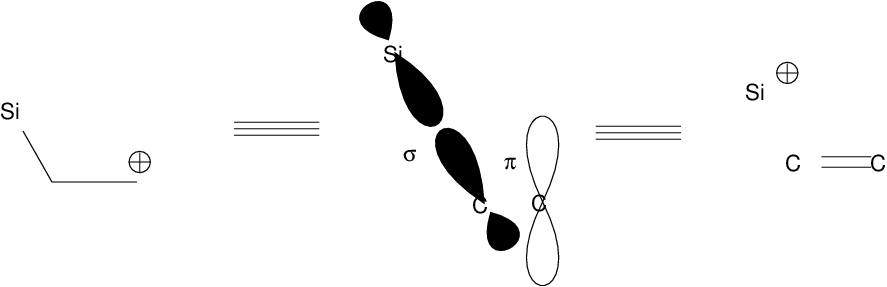
\includegraphics[width=0.7\textwidth]{img/intro/b-effect.png}}}\end{figure}
\end{block}
\pause
\begin{block}{$\alpha$ anioni: ($\sigma$*--p)$_\pi$}
\begin{figure}{\centering{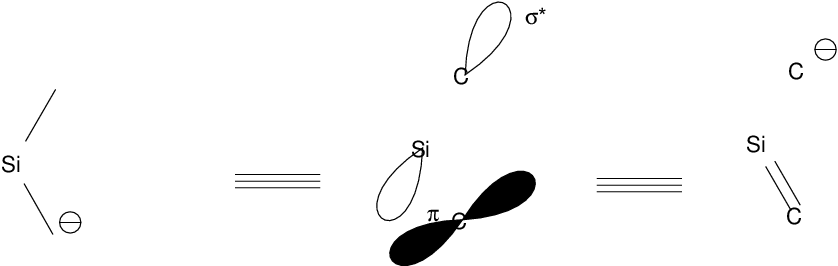
\includegraphics[width=0.7\textwidth]{img/intro/a-anions.png}}}\end{figure}
\end{block}
\end{frame}

\logo{
\includegraphics[width=0.07\paperwidth]{img/snslogo.png}}

%%%%%%%%%%%%%%%%%%%%%%%%%%%%%%%%%%%%%%%%%%%%%%%%%%%%%%%%%%%%%%%%%%%%

\diapo{Schema generale delle reazioni di interesse}
\begin{figure}{\centering{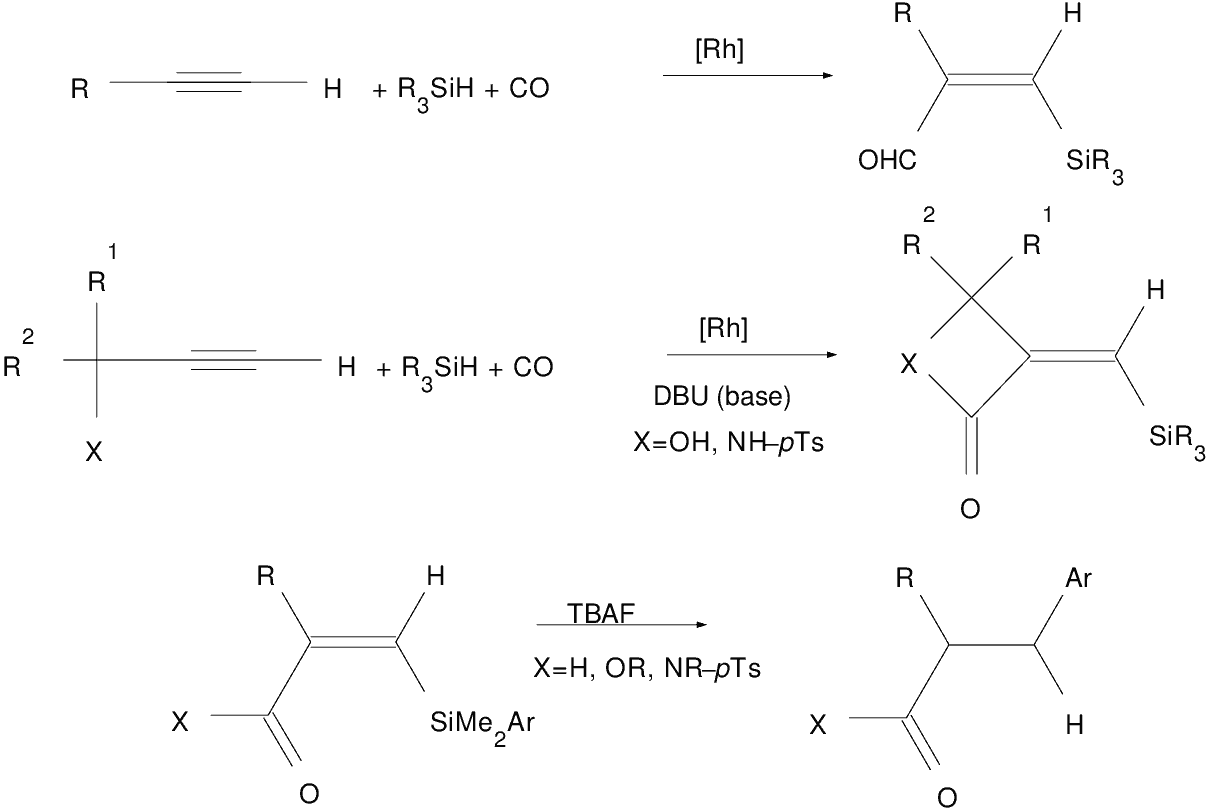
\includegraphics[width=0.8\textwidth]{img/intro/generale.png}}}\end{figure}


\end{frame}

\subsection{Prodotti ottenibili da $\beta$-silil alchenali}\begin{frame}\frametitle{Prodotti ottenibili da $\beta$-silil alchenali}
I $\beta$-sililalchenali ottenuti possono poi essere trasformati sfruttando la {\bf reattività sia di un carbonile $\alpha , \beta $ insaturo sia di un vinil silano}.
\begin{figure}{\centering{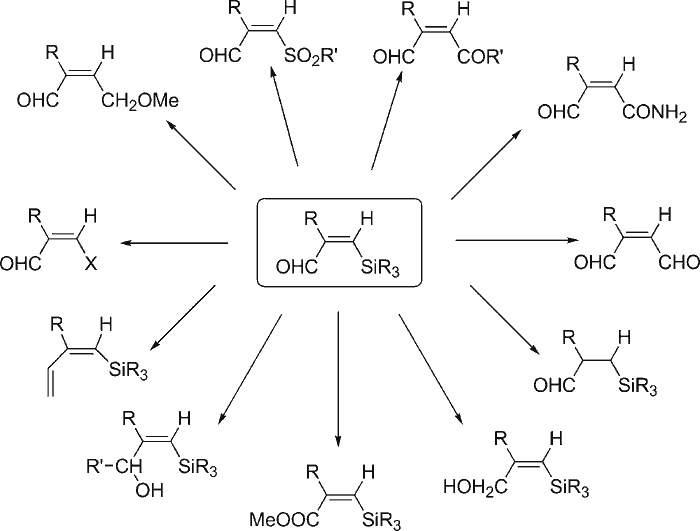
\includegraphics[width=0.6\textwidth]{img/intro/altri_prodotti_ottenibili.png}}}\end{figure}


\end{frame}


%%%%%%%%%%%%%%%%%%%%%%%%%%%%%%%%%%%%%%%%%%%%%%%%%%%%%%%%%%%%%%%%%%%%



%%%%%%%%%%%%%%%%%%%%%% Capitolo 2 %%%%%%%%%%%%%%%%%%%%%%
\input{Capitoli/sensibilizzatore}
%%%%%%%%%%%%%%%%%%%%%% Capitolo 3 %%%%%%%%%%%%%%%%%%%%%%
\input{Capitoli/catalizzatore}
%%%%%%%%%%%%%%%%%%%%%% Capitolo 4 %%%%%%%%%%%%%%%%%%%%%%
\chapter{Conclusions}
In this laboratory work we were able to prepare a \emph{tropos} chiral compound to use as chiral ligand for rhodium(I) in the addition of aryl\-boronic acids to 1-nitro-alkenes.

The strategy followed by our group for the homocoupling of 2-iodo-1-methoxy\-naphthalene was not successful because of a side reaction that can occur on methoxy\-naphthalene and not on methoxy\-benzenes, due to the presence of the $\alpha$' hydrogen.
As an alternative, using the Ullmann reaction, coupling was performed (by other groups) without problems and was possible to proceed with the subsequent steps to obtain the \emph{tropos} ligand \cmpd+{legante}.

The crucial step of the synthesis is reaction with \ce{PCl3} first with binaphthyl \cmpd+{dhn} and then with protected deoxychilic acid \cmpd{amda}. In this step working under inert atmosphere is a strict condition to avoid hydrolysis of \ce{PCl3}. %and derivatives that are not reactive towards our compounds. 
We obtained only 5~\% yield, so we can suppose that some moisture entered the reaction apparatus, probably during filtration of binaphthyl chloro\-phosphite and the transfer of this to the next reaction with \cmpd+{amda}.

Performing previous steps afforded pure compounds in modest to good yields after flash chromatography.

In the target enantio\-selective reaction we observed a poor conversion (17~\%) and the formation of 4 products: \emph{cis} (1\rS,2\rS), (1\Rs,2\Rs) and \emph{trans} (1\rS,2\Rs), (1\Rs,2\rS) [(1{\slshape ?},2{\slshape ?})-2-nitro-cyclo\-hexyl]benzene \cmpd+{ncb}. \emph{Trans} product was prevalent having a diastereo\-meric excess of 25~\%. The enantio\-meric excess of the \emph{trans} product was 60~\%.
%%%%%%%%%%%%%%%%%%%% Bibliografia %%%%%%%%%%%%%%%%%%%%%%
\bibliographystyle{unsrt}
\bibliography{inorganica2.bib}
\end{document}
